\documentclass[11pt,twoside,a4paper]{article}
% http://www-h.eng.cam.ac.uk/help/tpl/textprocessing/latex_maths+pix/node6.html symboles de math
% http://fr.wikibooks.org/wiki/Programmation_LaTeX Programmation latex (wikibook)
%=========================== En-Tete =================================
%--- Insertion de paquetages (optionnel) ---
\usepackage[french]{babel}   % pour dire que le texte est en fran{\'e}ais
\usepackage{a4}	             % pour la taille   
\usepackage[T1]{fontenc}     % pour les font postscript
\usepackage{epsfig}          % pour gerer les images
%\usepackage{psfig}
\usepackage{amsmath, amsthm} % tres bon mode mathematique
\usepackage{amsfonts,amssymb}% permet la definition des ensembles
\usepackage{float}           % pour le placement des figure
\usepackage{verbatim}

\usepackage{longtable} % pour les tableaux de plusieurs pages

\usepackage[table]{xcolor} % couleur de fond des cellules de tableaux

\usepackage{lastpage}

\usepackage{multirow}

\usepackage{multicol} % pour {\'e}crire dans certaines zones en colonnes : \begin{multicols}{nb colonnes}...\end{multicols} 

% \usepackage[top=1.5cm, bottom=1.5cm, left=1.5cm, right=1.5cm]{geometry}
% gauche, haut, droite, bas, entete, ente2txt, pied, txt2pied
\usepackage{vmargin}
\setmarginsrb{0.20cm}{0.20cm}{0.20cm}{0.20cm}{15pt}{3pt}{15pt}{3pt}

\usepackage{lscape} % changement orientation page
%\usepackage{frbib} % enlever pour obtenir references en anglais
% --- style de page (pour les en-tete) ---
\pagestyle{empty}

% % % en-tete et pieds de page configurables : fancyhdr.sty

% http://www.trustonme.net/didactels/250.html

% http://ww3.ac-poitiers.fr/math/tex/pratique/entete/entete.htm
% http://www.ctan.org/tex-archive/macros/latex/contrib/fancyhdr/fancyhdr.pdf
% \usepackage{fancyhdr}
% \pagestyle{fancy}
% % \newcommand{\chaptermark}[1]{\markboth{#1}{}}
% % \newcommand{\sectionmark}[1]{\markright{\thesection\ #1}}
% \fancyhf{}
% \fancyhead[LE,RO]{\bfseries\thepage}
% \fancyhead[LO]{\bfseries\rightmark}
% \fancyhead[RE]{\bfseries\leftmark}
% \fancyfoot[LE]{\thepage /\pageref{LastPage} \hfill
	% TITLE
% \hfill 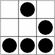
\includegraphics[width=0.5cm]{img/logo_glider.png} }
% \fancyfoot[RO]{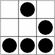
\includegraphics[width=0.5cm]{img/logo_glider.png} \hfill
	% TITLE
% \hfill \thepage /\pageref{LastPage}}
% \renewcommand{\headrulewidth}{0.5pt}
% \renewcommand{\footrulewidth}{0.5pt}
% \addtolength{\headheight}{0.5pt}
% \fancypagestyle{plain}{
	% \fancyhead{}
	% \renewcommand{\headrulewidth}{0pt}
% }


%============================= Corps =================================
\begin{document}

\setlength\parindent{0pt}

\texttt{http://blogs.rue89.nouvelobs.com/extension-du-domaine-du-jeu/2014/12/04/un-magasin-ikea-cest-construit-comme-un-jeu-video-233879}~\\

\textbf{\Large Un magasin Ikea, c'est construit comme un jeu vid{\'e}o} ~\\

\emph{\small par Oscar Barda --- Game designer, Publi{\'e} le 04/12/2014 {\`a} 17h38} ~\\

\begin{minipage}[ht]{0.65\textwidth}
	Vous ne voyez s{\^u}rement pas de prime abord le lien entre les magasins Ikea et les jeux vid{\'e}o... C'est bien normal : ~\\
	\begin{itemize}
    	\item l'un est bien r{\'e}el, consomme 1\% de la production mondiale de bois, {\'e}dite le catalogue le plus imprim{\'e} de la terre et meuble moult maisons, g{\'e}n{\'e}rant au passage des profits astronomiques ;
    	\item l'autre est virtuel, cens{\'e}ment sans cons{\'e}quence et sans incidence sensible sur le << vrai >>...
	\end{itemize}
	Quel rapport pourrait-il bien y avoir entre les deux ? %% ~\\
\end{minipage} \hfill \begin{minipage}[ht]{7.00cm}
	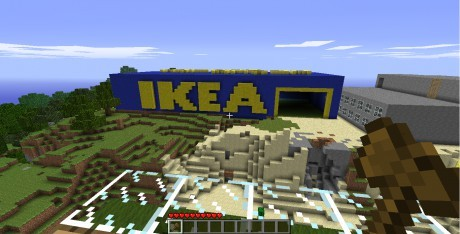
\includegraphics[width=6.95cm]{img/ikea.jpg}
	\emph{\footnotesize Capture d'{\'e}cran d'un magasin Ikea dans le jeu vid{\'e}o <<Minecraft>> }
\end{minipage}~\\~\\

Sans vouloir par trop flambax, examinons par l'optique du jeu vid{\'e}o le design de l'exp{\'e}rience Ikea et trouvons les passerelles et les diff{\'e}rences l{\`a} o{\`u} elles sont.~\\

Ce n'est pas pour rien qu'Ikea n'est pas Amazon, cherche {\`a} minimiser sa pr{\'e}sence en ligne ou {\`a} proposer des frais de port assez importants pour motiver l'acheteur potentiel {\`a} se d{\'e}placer : c'est parce qu'Ikea est le ma{\^i}tre incontest{\'e} du design de jeux vid{\'e}o dans le monde r{\'e}el. Oui.~\\

\textbf{\large Le level design, c'est architecturer un chemin}~\\

Dans un jeu vid{\'e}o, une fois les r{\`e}gles trouv{\'e}es, il faut passer {\`a} ce que l'on appelle le << level design >>, c'est-{\`a}-dire la mise en espace de ces r{\`e}gles et {\'e}l{\'e}ments de jeu.~\\

Par exemple, dans << Mario >>, le game designer dira << il existe dans ce monde des ennemis, des bonus, des trous et des pi{\`e}ges >>, et le level designer construira avec ces {\'e}l{\'e}ments des niveaux dont la courbe narrative (une salle pleine de cadavres par exemple construit une narration et une tension) et la courbe de difficult{\'e} (\c{c}a commence doucement et peu {\`a} peu, {\`a} mesure que je progresse, le jeu devient plus dur) sont parfaitement taill{\'e}s.~\\

Cette mise en place des {\'e}l{\'e}ments est {\`a} la fois un parcours lisible et lin{\'e}aire dont le joueur peut faire sens localement, sans pour autant le rendre trop intelligible globalement (l'environnement local et imm{\'e}diat du visiteur d'Ikea doit lui raconter une histoire mais ne doit pas lui r{\'e}v{\'e}ler toute la trame du magasin).~\\

\textbf{\large Un labyrinthe efficace}~\\

Un bon constructeur d'Ikea et un bon level designer doivent tous deux construire un labyrinthe efficace : un d{\'e}dale dans lequel il fait bon {\^e}tre, dans lequel on a une furieuse impression d'avoir son libre arbitre, de pouvoir choisir o{\`u} l'on va et o{\`u} l'on reste, mais o{\`u} cette impression est fausse et biais{\'e}e car l'espace est si bien sculpt{\'e} que m{\^e}me les barreaux dor{\'e}s de notre prison sont invisibles.~\\

Ikea construit << le long cheminement naturel >>, ce sinueux lacis de pi{\`e}ces et d'ambiances dans lequel on aime tant se perdre, se laisser porter par le lent flux des autres visiteurs. Le chemin doit tourner environ tous les 15 m, sinon le plan du magasin devient bien trop {\'e}vident, il doit traverser des espaces tr{\`e}s contrast{\'e}s pour donner l'impression de la variabilit{\'e} et surtout dissimuler sa nature lin{\'e}aire.~\\

Comme le jeu vid{\'e}o, Ikea doit construire sans cesse de nouveaux points de vues, de nouvelles ambiances, sentiments et espaces. C'est ce qu'on appelle l'{\'e}conomie de l'attention, et si l'on se rend compte qu'on est pi{\'e}g{\'e} et men{\'e} par le bout du nez, Ikea a perdu. C'est le pire cauchemar des architectes d'Ikea : l'<< autobahn >> ou autoroute ; c'est pour eux une id{\'e}e d{\'e}testable car elle permettrait au client de litt{\'e}ralement passer {\`a} c{\^o}t{\'e} d'objets qu'ils auraient pu d{\'e}couvrir et surtout, lorsqu'ils ont trouv{\'e} ce qu'ils voulaient, de courir directement {\`a} la sortie.~\\

\textbf{\large Architecturer le shopping comme un jeu}~\\

Non, il faut que vous soyez pris par le rythme des autres, le courant g{\'e}n{\'e}ral de la foule et que comme elle, lentement, vous chemini... Oh mais t'as vu cette petite lampe, elle co{\^u}te comb... 10 balles ? ! On la prend !~\\

C'est l{\`a} tout le d{\'e}fi d'Ikea, le d{\'e}fi de tout commer\c{c}ant, en fait, qui d{\'e}passe une certaine quantit{\'e} d'objets {\`a} son inventaire : la d{\'e}couvrabilit{\'e}. Comment font YouTube, Apple, Amazon pour mettre en avant, pour faire d{\'e}couvrir, pour montrer les millions d'objets de leurs catalogues ? Ikea a la r{\'e}ponse : on architecture le shopping comme un jeu.~\\

\c{C}a n'est pas tant qu'Ikea fait un jeu ou que << la vie est un jeu >>, c'est que le jeu et en particulier le jeu vid{\'e}o se joue de nous avec une dext{\'e}rit{\'e} d{\'e}concertante. Apr{\`e}s vingt ans {\`a} peaufiner leur compr{\'e}hension de ce qu'est la nature humaine, ses envies et ses pulsions, les designers de jeu vid{\'e}o commencent {\`a} comprendre ce qui nous tire en avant, ce qui motive ou ennuie, et ils s'en servent comme d'une arme pour nous divertir (et pas seulement, nous y reviendrons).~\\

\textbf{\large Les achats impulsifs}~\\

\begin{minipage}[ht]{0.65\textwidth}
	Environ 60\% des ventes d'Ikea sont des achats impulsifs ou en tout cas << au-del{\`a} des intentions d'achats d'origine >>. C'est cela le pouvoir d'Ikea, de nous faire voyager, de nous faire vivre l'espace autrement pour nous y faire r{\^e}ver et a fortiori, pour nous y faire acheter.~\\

	Non, Ikea ne vous facilite pas la t{\^a}che : vous voulez une chaise ? Il va vous falloir traverser tout le magasin, rencontrant {\'e}videmment le long du chemin des objets que vous vouliez sans le savoir. Oui, dans les grandes all{\'e}es de Monoprix, il est bien courant de passer {\`a} c{\^o}t{\'e} de la moiti{\'e} de sa liste de cour... << RAAAH J'AI ENCORE OUBLI{\'E} DE RACHETER DU PQ ! >>~\\

	Chez Ikea c'est exactement l'inverse : au point que vous en oublieriez m{\^e}me peut-{\^e}tre que vous avez d{\'e}j{\`a} tel ou tel objet...~\\
\end{minipage} \hfill \begin{minipage}[ht]{7.00cm}
	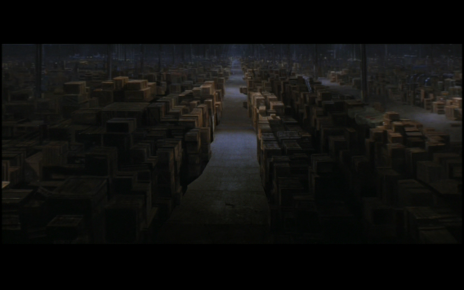
\includegraphics[width=6.95cm]{img/raiders_of_the_lost_ark.png}
	\emph{\footnotesize << Bordel c'est o{\`u} le rayon lampes ? ! >>. Capture d'{\'e}cran du film << Indiana Jones et les aventuriers de l'arche perdue >>, de Steven Spielberg, 1981}~\\
\end{minipage}~\\~\\

\textbf{\large Influencer, l'air de ne pas y toucher}~\\

Dans le jeu << Half-Life 2 >>, les cr{\'e}ateurs du jeu avaient {\`a} un moment cr{\'e}{\'e} et anim{\'e} une sc{\`e}ne tr{\`e}s complexe : le crash d'un vaisseau extra-terrestre dans une structure. Seulement un probl{\`e}me s'est vite pos{\'e} : et si le joueur ne regarde pas au bon moment ? Dans un jeu {\`a} la premi{\`e}re personne, le joueur contr{\^o}le son point de vue (la cam{\'e}ra) et s'il regarde {\`a} c{\^o}t{\'e} au moment du crash, nous avons pass{\'e} trois semaines {\`a} animer m{\'e}ticuleusement la sc{\`e}ne pour rien... Forcer la cam{\'e}ra {\`a} regarder par l{\`a} ? Non, inutile de reprendre le contr{\^o}le au joueur ou de lui dicter les choses, mieux vaut manipuler le niveau...~\\

Au moment opportun, un ennemi se met {\`a} vous tirer dessus de tr{\`e}s haut, il vous canarde et vous ne pouvez pas avancer en terrain d{\'e}couvert. Vous dissimulant derri{\`e}re un tas de d{\'e}bris, vous vous mettez {\`a} r{\'e}pliquer, et au moment o{\`u} vous le touchez un vaisseau alien d{\'e}barque dans l'{\'e}cran et s'{\'e}crase dans la structure...~\\

Oui, les designers de << Half-Life 2 >> sont malins, ils n'ont pas besoin de vous forcer {\`a} regarder, ils n'ont qu'{\`a} mettre un danger {\`a} cet endroit, un objectif, une cible, et {\`a} d{\'e}clencher leur sc{\`e}ne au moment o{\`u} ils peuvent {\^e}tre certains que vous y faites attention : au moment l'ennemi prend des d{\'e}g{\^a}ts, au moment o{\`u} vous lui tirez dessus.~\\

Ikea fonctionne de fa\c{c}on similaire, traverser les espaces, les mettre en lumi{\`e}re, rendre leur fonctionnalit{\'e} {\'e}vidente dans un contexte donn{\'e}... Tomber face {\`a} une petite lampe trop mignonne au d{\'e}tour d'une all{\'e}e, exister dans une pi{\`e}ce, donne une id{\'e}e bien plus poignante qu'une photo fond blanc sur papier glac{\'e} qu'on aurait laiss{\'e}e bien rang{\'e}e dans la cat{\'e}gorie << lampe >> du catalogue.~\\

\textbf{\large Coproduire la valeur}~\\

Dans << Minecraft >>, dans << Les Sims >>, dans << Civilisation >>, ou dans un << Tamagotchi >>, le joueur cr{\'e}e quelque chose, il transmet {\`a} la machine une intention. Cette intervention, le jeu ou l'ordinateur la retient : j'{\'e}tais l{\`a}, j'ai fait \c{c}a, j'y ai pass{\'e} du temps et ce temps a de la valeur pour moi. Monter un meuble Ikea, c'est avoir une main dans sa fabrication, dans son assemblage, c'est coproduire la valeur {\'e}motionnelle d'un objet et lui adjoindre une histoire, celle de sa construction, c'est d{\'e}j{\`a} lui donner vie.~\\

Cette m{\'e}canique est {\'e}videmment renforc{\'e}e par le refus strict d'Ikea de nommer les objets << chaise >> ou << table >> non, ce sont des << PR{\"U}NTZ ou des SHTR\O K (noms non contractuels) toujours {\'e}crits en majuscule. Ils ne sont pas des objets ordinaires et intellectuellement, nous donnons plus de valeur aux objets que nous devons travailler pour obtenir qu'{\`a} ceux qu'on r{\'e}cup{\`e}re d{\'e}j{\`a} faits.~\\

Dans <<World of Warcraft>>, la qu{\^e}te de l'ouverture des portes d'Ahn Qiraj, le donjon des sables, prenait {\`a} sa sortie des dizaines d'heures {\`a} finir : il fallait rassembler 40 joueurs (oui, 40 personnes) et les faire m{\'e}ticuleusement travailler ensemble pour r{\'e}cup{\'e}rer des objets des quatre coins du jeu pour enfin avoir droit de passer les portes monumentales du temple.~\\

Et qu'y trouvaient donc les braves aventuriers ? Une <<{\'e}p{\'e}e>> ? Une <<cape>> ? Un <<bijou>> ? Non point ! Ils y trouvaient <<la lame de Kalimdor>>, <<le vestement de l'oracle>> ou <<l'anneau des dieux anciens>>. Donner une valeur {\`a} l'objet, c'est aussi lui attribuer un nom qui diff{\`e}re de sa fonction, un nom qui permettra de d{\'e}signer son unicit{\'e} et les circonstances particuli{\`e}res de son obtention ou de sa fabrication.~\\

%% Les portes d'Ahn Qiraj %% WoW (World of Warcraft)
%% Un {\'e}v{\'e}nement du monde du jeu vid{\'e}o. Et pendant ce temps-l{\`a} y'a Anne qui rage.

Toutefois il faut {\'e}quilibrer savamment ce moment d'obtention : s'il est trop complexe, autant fabriquer un meuble soi-m{\^e}me et Ikea vous fait perdre votre temps, vous ne rejouerez jamais {\`a} ce jeu ; s'il est trop simple par contre, vous n'aurez pas le plaisir d'avoir vous-m{\^e}me <<fabriqu{\'e}>> ce meuble. Ikea travaille savamment et d{\'e}lib{\'e}r{\'e}ment ce rapport temps investi -- valeur {\'e}motionnelle.~\\

\textbf{\large Le langage sans la langue}~\\

Un dernier {\'e}l{\'e}ment qu'Ikea manipule avec brio : un langage international qui se passe de mots. Si les raisons de l'absence d'instruction {\'e}crites dans les manuels de montage des meubles Ikea existent (le fondateur de la compagnie est dyslexique et traduire les manuels dans toutes les langues co{\^u}terait cher en papier et en encre), la marque su{\'e}doise n'en cr{\'e}e pas moins un langage, une forme de communication avanc{\'e}e, permettant {\`a} tous et {\`a} chacun de r{\'e}soudre le puzzle, de jouer {\`a} assembler son meuble sans le verbaliser. Vous savez qui d'autre fait \c{c}a ? Lego et ses manuels de montage {\'e}tape par {\'e}tape.~\\

Les jeux et les jouets communiquent sans mot, disent des choses {\`a} tous les {\^e}tres humains, peu importe leur sexe, leur race ou leur origine... Par le basket-ball, deux {\'e}quipes de deux pays diff{\'e}rents peuvent avoir une conversation, {\'e}changer des passes, des feintes, des sourires, des cris et des {\'e}motions sans jamais s'{\^e}tre pr{\'e}c{\'e}demment connues et sans faire m{\^e}me une phrase. Les jeux peuvent m{\^e}me franchir un pas de plus et communiquent au-del{\`a} des esp{\`e}ces :~\\

Un crapaud qui joue {Vid{\'e}o}... --- <<Une grenouille vit un iPhone qui lui sembla de belle taille.>>~\\

Et vous, quand jouerez-vous donc {\`a} un jeu vid{\'e}o avec votre chat ? Et cela modifiera t-il vos relations {\`a} votre animal de compagnie ?~\\

\textbf{\large Design du capitalisme}~\\

\begin{minipage}[ht]{7.00cm}
	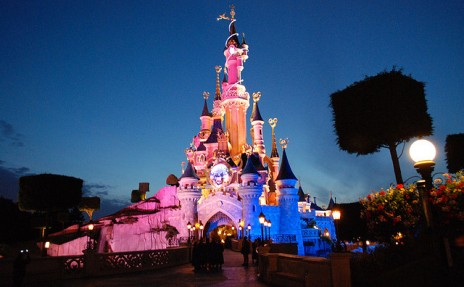
\includegraphics[width=6.95cm]{img/3620468272_02ffb32bfb_z-1_0.jpg}
	\emph{\footnotesize Le ch{\^a}teau de Disneyland Paris, illumin{\'e} la nuit (Sam Lavy/Flickr/CC)}~\\
\end{minipage} \hfill \begin{minipage}[ht]{0.65\textwidth}
	Ikea est construit sur des principes de design utilitaire ; la compagnie utilise l'architecture comme un outil du capitalisme pour vous faire acheter, de la m{\^e}me fa\c{c}on que les jeux dits <<gratuits>> sur mobile utilisent l'art du jeu pour vous faire d{\'e}penser de l'argent. Mais l'architecture comme le jeu peuvent aspirer {\`a} de bien plus belles fonctions -- chacun d{\'e}cidera pour lui s'il les trouve plus nobles -- mais le jeu, ses recherches et ses trouvailles sur la nature des humains restent un outil puissant qui ne servira que les buts qu'on voudra bien lui faire servir. Il existe Ikea et la tour Eiffel, <<Small Worlds>> et <<Candy Crush>>.~\\

	Qui d'autre s'est {\`a} votre avis rendu compte que le jeu et l'espace pouvaient se jouer de vous ? Quel autre exemple de parangon de l'architecture manipulatrice habite notre beau pays ?~\\
\end{minipage} ~\\~\\

Disneyland. Et oui, si Ikea est si proche du jeu, c'est aussi qu'Ikea est proche du parc d'attraction dans sa fa\c{c}on de penser l'espace dans sa dualit{\'e} entre contrainte et libert{\'e} per\c{c}ue.~\\

Mais si le jeu peut biaiser, guider, mener par le bout du nez... Peut-il r{\'e}ellement manipuler jusque dans le monde r{\'e}el ? Voil{\`a} le sujet d'un prochain article !~\\

\end{document}
